%%%%%%%%%%%%%%%%%%%%%%%%%%%%%%%%%%%%%%%%%%%%%%%%%%%%%%%%%%%%%%%%%%%%%%%%%%%
% Definitions                                                             %
%%%%%%%%%%%%%%%%%%%%%%%%%%%%%%%%%%%%%%%%%%%%%%%%%%%%%%%%%%%%%%%%%%%%%%%%%%%
\gdef\version{1.0}  % do not forget to update this
\gdef\doctype{Technische Dokumentation}


%%%%%%%%%%%%%%%%%%%%%%%%%%%%%%%%%%%%%%%%%%%%%%%%%%%%%%%%%%%%%%%%%%%%%%%%%%%
% This section defines the template.                                      %
% DO NOT CHANGE ANYTHING IN THE SECTION                                   %
%%%%%%%%%%%%%%%%%%%%%%%%%%%%%%%%%%%%%%%%%%%%%%%%%%%%%%%%%%%%%%%%%%%%%%%%%%%
% For correct typesetting you will need the following fonts:              %
% - Roboto                                                                %
% - Adobe Garamond Pro                                                    %
% - EB Garamond Regular SmallCaps                                         %
%%%%%%%%%%%%%%%%%%%%%%%%%%%%%%%%%%%%%%%%%%%%%%%%%%%%%%%%%%%%%%%%%%%%%%%%%%%

\documentclass[12pt, letterpaper]{report}
\usepackage[hmargin=1in,vmargin=1.5in]{geometry}
\usepackage[T1]{fontenc}
\usepackage[T1]{fontenc}
\usepackage[ngerman]{babel}
\usepackage{graphicx}
\usepackage{fontspec,xunicode}
\usepackage{sectsty}
\usepackage{tabu}
\usepackage{fancyhdr}
\usepackage{titlesec}
\usepackage{url}
\usepackage{lastpage}
\usepackage{float}
\usepackage[ngerman]{babel}
\usepackage[official]{eurosym}
\usepackage{listings}


\usepackage[
	colorlinks,
	citecolor=black,
	filecolor=black,
	linkcolor=black,
	urlcolor=black,
	linktoc=all
]{hyperref}

\allsectionsfont{\fontspec{Roboto Condensed Light}}
\defaultfontfeatures{Mapping=tex-text,Scale=MatchLowercase}
\setmainfont{Adobe Garamond Pro}
\setmonofont{Source Code Pro}

\setlength{\topskip}{0mm}
\setlength{\parskip}{1em}
\setlength{\parindent}{0em}

\usepackage{enumitem}\setlist{nolistsep}


\titleclass{\chapter}{straight}
\titleformat{\chapter}[hang]{\Huge\bfseries}{\fontspec{Roboto Condensed Light}\thechapter.}{10pt}{\fontspec{Roboto Condensed Light}\Huge\bfseries}

\titlespacing*{\chapter}{0pt}{1cm}{0pt}
\titlespacing*{\section}{0mm}{5mm}{0pt}

\renewcommand{\arraystretch}{2}

%\setlength{\voffset}{2cm}

% headers
\renewcommand{\headrulewidth}{0.4pt}
\renewcommand{\footrulewidth}{0.4pt}
\fancyhead{}
\fancyfoot{}
\pagestyle{fancy}
\lhead{Naschmarkt \em{\doctype}\\}
\rhead{\small{Markus Klein, Thomas Fellner, \\Matthias Schwebler, Philip Vonderlind}}

\lfoot{Version \version}
\rfoot{\thepage\ von \pageref{LastPage}}
\setlength{\headheight}{30pt}

\lstset{
	basicstyle=\ttfamily\small,
	keywordstyle=\bfseries\color[rgb]{0.496,0.000,0.332},
	commentstyle=\color[rgb]{0.246,0.496,0.371},
	stringstyle=\color[rgb]{0.164,0.000,0.996},
	tabsize=4,
	breaklines=true,
	numbers=left,
	numberstyle=\tiny\color{black},
	stepnumber=2,
	numbersep=8pt,
	numberstyle=\tiny,
	captionpos=b,
	xleftmargin=1cm,
	showspaces=false,
	showstringspaces=false,
	basewidth={0.53em,0.45em},
	frame=single,
	xleftmargin=1cm,
	basicstyle=\scriptsize,
}

%%%%%%%%%%%%%%%%%%%%%%%%%%%%%%%%%%%%%%%%%%%%%%%%%%%%%%%%%%%%%%%%%%%%%%%%%%%
% Document Start                                                          %
%%%%%%%%%%%%%%%%%%%%%%%%%%%%%%%%%%%%%%%%%%%%%%%%%%%%%%%%%%%%%%%%%%%%%%%%%%%

\begin{document}
	\begin{titlepage}
		\begin{center}
			\vspace*{1cm}

			{\fontsize{25}{25}\fontspec{EB Garamond Regular SmallCaps} Naschmarkt\\}
            \vspace{0.3cm}
            {\fontsize{25}{25}\fontspec{EB Garamond Regular SmallCaps}{\large Technische Dokumentation}}

			\vspace{2.5cm}

			2016 - 4BHIT

			\vspace*{5mm}

			\small{Markus Klein, Thomas Fellner,\\Matthias Schwebler, Philip Vonderlind}

			\vspace*{2cm}

			Version \version

			\vfill

			\chapter*{Freigabe}
			\begin{center}
				\begin{tabu} to \textwidth { | @{\hspace{3mm}} l @{\hspace{3mm}} | @{\hspace{3mm}} l | @{\hspace{3mm}} l @{\hspace{3mm}} | X[l] | }
					\hline
					& Name & Datum & Unterschrift \\ \hline
					Erstellt: & M. Klein, T. Fellner & 18.1.2016 & \\ \hline
					Gepr\"uft: & M. Schwebler, P. Vonderlind & 19.1.2016 & \\ \hline
					Freigegeben: &  &  & \\
					\hline
				\end{tabu}
			\end{center}

		\end{center}
	\end{titlepage}


	\newpage
	\tableofcontents


	\newpage
	\chapter*{Einf\"uhrung}

    \chapter{Systemanforderungen}
    Bei dem Naschmarkt handelt es sich um eine in PHP implementierte Webapplikation, dabei ergeben sich folgende Systemanforderungen:
\begin{itemize}
    \item PHP >= 5.5.9
    \item OpenSSL PHP Extension
    \item PDO PHP Extension
    \item Mbstring PHP Extension
    \item Tokenizer PHP Extension
    \item Datenbankserver: Der Naschmarkt \"unterst\"utzt folgende Datenbankserver (Test wurden ausschlie\ss lich mit MySQL durchgef\"uhrt)
        \begin{itemize}
            \item MySQL
            \item Postgres
            \item SQLite
            \item SQL Server
        \end{itemize}
\end{itemize}

\section{Entwicklungsanforderungen}


    \chapter{Installation}
    \section{Installation vorbereiten}
Bevor die Applikation auf das Zielsystem ausgeliefert werden kann, muss der Naschmarkt zur Installation bereit gemacht werden.
In diesem Schritt werden Abh\"angigkeiten installiert und verschiedenste Buildprozesse ausgef\"uhrt.
Dieser Schritt kann sowohl auf dem lokalen Host als auch dem Zielserver erfolgen.

Daf\"ur werden aus dem Projektverzeichnis folgende Kommandos ausgef\"uhrt:
\begin{lstlisting}[caption=Installationsvorbereitung]
# Install composer (PHP) dependencies
composer install

# Install frontend and JavaScript dependencies
npm install

# Run build tasks
gulp
\end{lstlisting}

\section{Konfiguration}
Um den Naschmarkt zu konfiguration muss eine Umgebunskonfiguration (Environment) erstellt werden.
F\"ur diese Konfigurationsdatei gibt es im Hauptverzeichnis ein Beispiel namens \texttt{.env.example}.

\begin{lstlisting}[caption=Beispielenvironment]
# no need to change this
APP_ENV=local
APP_DEBUG=true
APP_KEY=SomeRandomString

# database configuration
DB_HOST=127.0.0.1
DB_DATABASE=homestead
DB_USERNAME=homestead
DB_PASSWORD=secret

# no need to change this
CACHE_DRIVER=file
SESSION_DRIVER=file
QUEUE_DRIVER=sync

# Mail configuration
# See https://laravel.com/docs/5.2/mail#introduction for details
MAIL_DRIVER=smtp
MAIL_HOST=mailtrap.io
MAIL_PORT=2525
MAIL_USERNAME=null
MAIL_PASSWORD=null
MAIL_ENCRYPTION=null
\end{lstlisting}
Diese wird nach \texttt{.env} kopiert und entsprechend bearbeitet.
Weitere Konfigurationsparameter befinden sich in den Dateien des \texttt{config} Ordners, diese sollten unter normalen Umst\"anden jedoch keiner Anpassung bed\"urfen.
F\"ur eine genauere Beschreibung sei an die Konfigurationsdokumentation von Laravel unter \url{https://laravel.com/docs/5.2/configuration} verwiesen.
Danach muss noch ein Application Key generriert werden, dies erfolgt mit folgendem Befehl:

\begin{lstlisting}[caption=Generieren des Applikationsschl\"ussels]
php artisan key:generate
\end{lstlisting}

Je nachdem, wo das Vorbereitung erfolgt ist, muss sp\"atenstens jetzt der Naschmarkt auf den Server hochgeladen werden.
Der Webroot des Webservers soll dabei auf das \texttt{public} Verzeichnis zeigen.


    \chapter{Applikationsstruktur}
    Da der Naschmarkt in dem Framework Laravel geschrieben ist, folgt es dem MVC Prinzip.

\begin{figure}[H]
	\begin{center}
		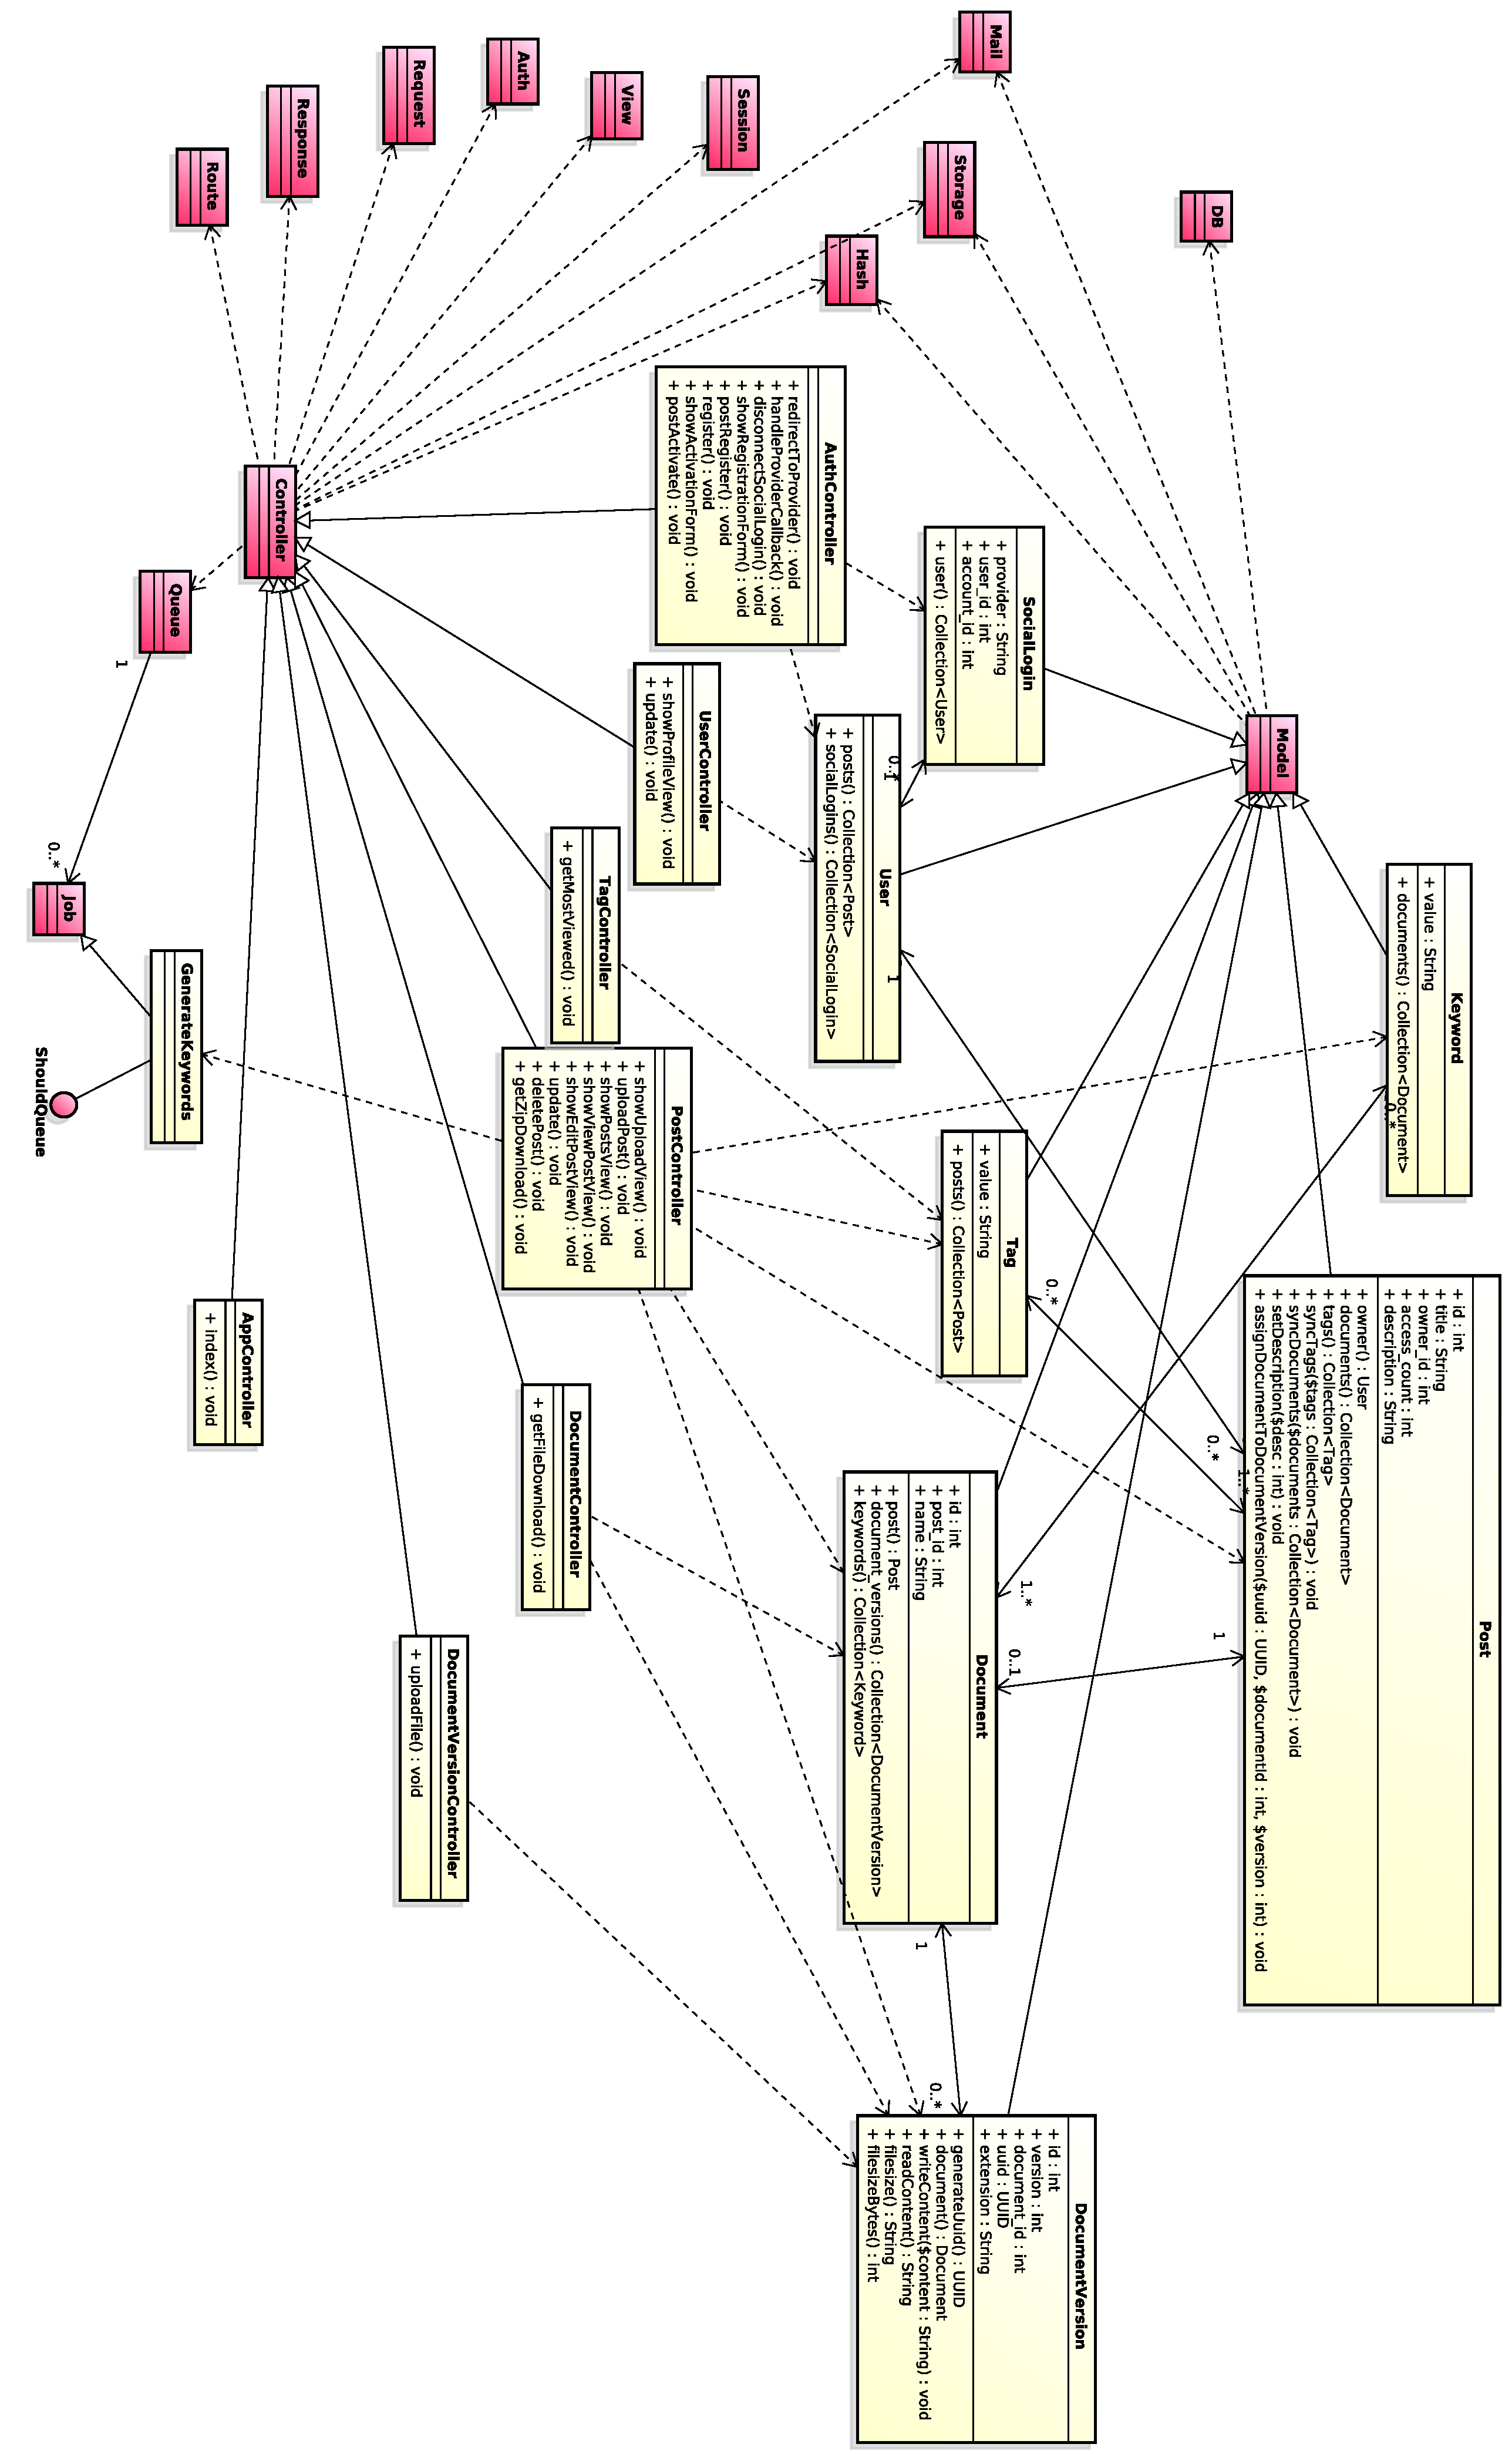
\includegraphics[width=\linewidth]{images/UML_Classdiagramm.pdf}
		\caption{UML Diagramm}
	\end{center}
\end{figure}

In der folgenden Graphik sind die M\"oglichkeiten des Projektes beschrieben in einem Use-Case Diagramm.

\begin{figure}[H]
	\begin{center}
		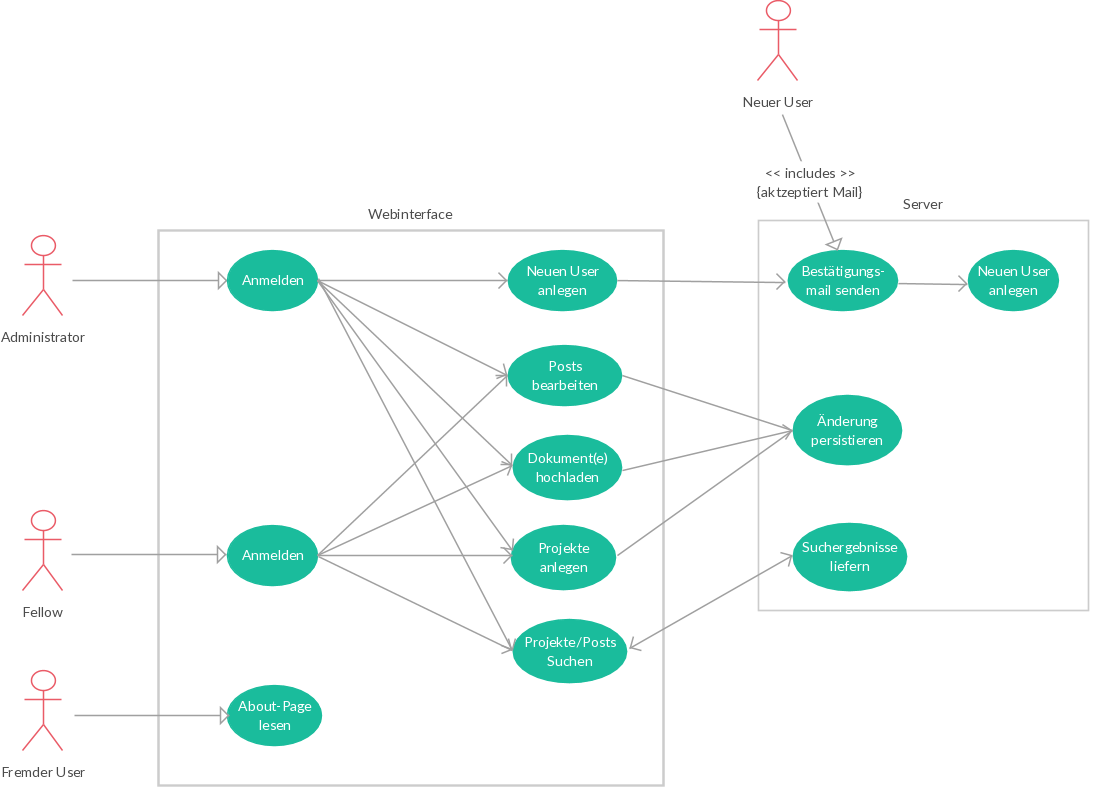
\includegraphics[width=\linewidth]{images/use_case.png}
		\caption{Use Case Diagramm}
	\end{center}
\end{figure}


    \chapter{Datenbankstruktur}
    Folgendes Entity Relationship (ER) Diagramm zeigt die Datenstruktur des Projektes:
\begin{figure}[H]
	\begin{center}
		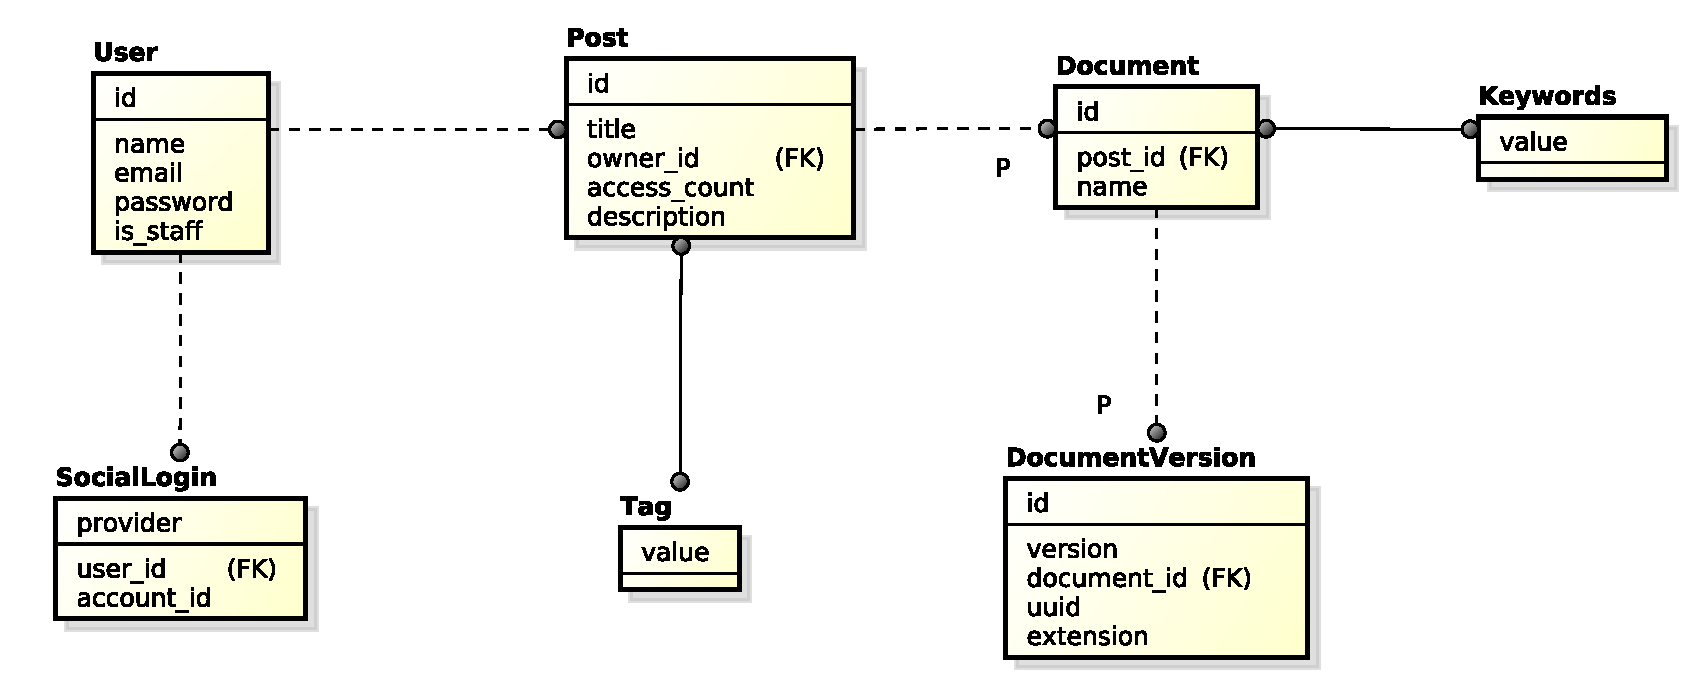
\includegraphics[width=\linewidth]{images/Datenstruktur.pdf}
		\caption{ER Diagramm}
	\end{center}
\end{figure}

\section{Weiterentwicklung}
Die Entwicklung und Versionierung der Datenbank erfolgt mit Migrationen.
Dabei handelt es sich um eine Funktionalit\"at des eingesetzten Frameworks, die Datenstruktur eines Projektes zu verwalten und entwickeln.

Hier ein Beispiel einer Migration, welche eine User Tabelle definiert.
\begin{lstlisting}[language={PHP}, caption=Beispiel eine Migration]
class CreateUsersTable extends Migration
{
  // Run the migrations.
  public function up()
  {
      Schema::create('users', function (Blueprint $table) {
          $table->increments('id');
          $table->string('name');
          $table->string('email')->unique();
          $table->string('password', 60);
          $table->rememberToken();
          $table->timestamps();
      });
  }

  // Reverse the migrations.
  public function down()
  {
      Schema::drop('users');
  }
}
\end{lstlisting}

Eine Migration wird erstellt mittels \texttt{php artisan create:migration [name]} und ist dann unter dem Ordner \texttt{database/migrations} mit allen bisherigen Migrationen zu finden und zu editieren.
Um dann die Datenbank zu migrieren (Datenstruktur in der Datenbank erstellen, nicht zu verwechseln mit dem erstellen Migrationsscript) wird der Befehl \texttt{php artisan migrate} ausgef\"uhrt.

Eine genauere Dokumentation zu Migrationen in Laravel ist in der offiziellen Dokumentation von Laravel unter \url{https://laravel.com/docs/5.2/migrations} zu finden.


    \chapter{Migrationsscript}
    Die Migration wird \"uber 2 in Python 2.7 geschriebenes Skripts abgehaldelt, welches die aus der aktuellen Wordpress Datenbank nimmt und sie auf die neue Datenstruktur umwandelt.
Zuerst sollte das Skript, welches die Benutzer migriert ausgef\"uhrt werden und dann das Skript welche alle Posts migriert.

\section{Ben\"otigte Bibliotheken}
Um das Skript ausf\"uhren zu k\"onnen, m\"ussen folgende Python Bibliotheken am ausf\"uhrenden Computer installiert sein.

\begin{itemize}
  \item \href{http://mysql-python.sourceforge.net/MySQLdb.html}{ \texttt{MySQLdb} }, welche jeweils zum Holen und Schreiben der Daten von der MySQL Datenbank verwendet wird
  \item \href{https://textract.readthedocs.io/en/latest/}{ \texttt{textract} }, welches f\"ur die Volltext-Suche die Datein indexiert
\end{itemize}

Das Skript wird dann \"uber die Kommandozeile mit \texttt{python} oder \texttt{python2.7 migrateUsers} oder \texttt{migrate Posts}

\section{Konfigurations Datei}
Das Skript kommt mit einer Konfigurationsdatei \texttt{config.py}, in welcher man die ben\"otigten Daten f\"ur

\begin{itemize}
  \item die alte Datenbank, woher die Daten kommen
  \item die neue Datenbank, wohin die Daten gespeichert werden
  \item den FTP Zugang um die Datein zu speichern\\
\end{itemize}

Hier ein Beispiel f\"ur das config file
\\
\begin{lstlisting}[language={Python}, caption=config.py]
"""

This is the config file for the Migration

There are 3 things to configure.
    - the old Database to migrate from
    - the new Database to save the migration
    - FTP connection to save the files

"""

# Old Database.
# This is where the Data is taken from
dbOld = {
    'host':         "mysql003.tophosting.at",   # host ip
    'port':         3306,                       # port
    'user':         "dbue88a3f4",               # username
    'password':     "Khy?8k9p",                 # password
    'database':     "dbf26d5267"                # name of
                                                # the database
}

# New Database.
# This is where the Data will be stored
dbNew = {
    'host':         "127.0.0.1",                # host ip
    'port':         33060,                      # port
    'user':         "homestead",                # username
    'password':     "secret",                   # password
    'database':     "homestead"                 # name of
                                                # the database
}

# FTP connection to save the files
ftpConnection = {
    'host':         "192.168.10.10",            # host ip
    'user':         "vagrant",                  # username
    'password':     "vagrant",                  # password
    'directory':    "naschmarkt/storage/app"    # directory where
                                                # to save the
                                                # files to
}
\end{lstlisting}

\end{document}
